\section{Introducción}

El ajuste entre las características de la persona y las demandas y oportunidades de su entorno laboral constituye un predictor central de múltiples resultados organizacionales. La teoría del ajuste persona--entorno (Person--Environment Fit, P-E Fit) sostiene que el grado de compatibilidad entre individuo y contexto explica de manera importante el estrés, el bienestar y una amplia gama de actitudes y conductas laborales \cite{edwards_person-job_1991,kristofBrown2005}. Desde una perspectiva integradora, esta teoría postula que los individuos buscan activamente entornos congruentes con sus características personales y que, cuando logran dicha correspondencia, experimentan consecuencias positivas tanto a nivel psicológico como conductual \cite{edwards1999}.

Dentro de este marco conceptual amplio, el ajuste persona--trabajo (Person--Job Fit, P-J Fit) se define como el grado de compatibilidad entre las características del individuo habilidades, conocimientos, valores, rasgos de personalidad y necesidades y las características del puesto demandas técnicas, recompensas, cultura organizacional y oportunidades de desarrollo \cite{edwards_person-job_1991,kristofBrown2005}. Este constructo se operacionaliza mediante dos formulaciones complementarias que capturan distintas facetas de la congruencia. La primera es el ajuste demandas--habilidades (Demands--Abilities, D-A), centrado en la correspondencia entre las competencias técnicas del individuo y las exigencias funcionales del rol. Este tipo de ajuste refleja si el trabajador posee las capacidades necesarias para cumplir con las responsabilidades del puesto de manera eficaz \cite{Cable2002}. La segunda formulación es el ajuste necesidades--suministros (Needs--Supplies, N-S), enfocado en la correspondencia entre lo que la persona valora o necesita por ejemplo, autonomía, reconocimiento, desarrollo profesional, equilibrio vida-trabajo y lo que el puesto provee en términos de recompensas intrínsecas y extrínsecas \cite{edwards1999}.

La evidencia empírica acumulada en las últimas dos décadas ha documentado de manera consistente que un alto P-J Fit se asocia con múltiples resultados organizacionales deseables: mayor satisfacción laboral, compromiso organizacional, desempeño en el rol, conductas de ciudadanía organizacional y bienestar psicológico, así como con menor intención de renuncia, ausentismo, estrés laboral y conflicto trabajo-familia \cite{kristofBrown2005}. Metaanálisis recientes confirman que el P-J Fit explica entre el 10\% y el 25\% de la varianza en satisfacción laboral e intención de renuncia, dependiendo de la operacionalización del constructo y las características de la muestra \cite{Cable2002,kristofBrown2005}.

Sin embargo, la mayoría de los estudios previos han tratado el P-J Fit como un constructo unidimensional o han agregado sus componentes técnicos y socioculturales, lo que limita la comprensión de los mecanismos específicos por los cuales distintas facetas del ajuste influyen sobre las actitudes y conductas laborales. Investigaciones recientes con diseño multivariado han comenzado a diferenciar entre el ajuste de habilidades (que refleja la correspondencia técnica entre competencias y demandas) y el ajuste de personalidad o valores (que refleja la compatibilidad sociocultural con el entorno del puesto), demostrando que ambos tipos de ajuste explican varianza única en resultados organizacionales y operan a través de procesos psicológicos parcialmente distintos \cite{lauver2001,Cable2002}.

Adicionalmente, diversos estudios confirman que los empleados diferencian claramente entre el ajuste con el puesto (P-J Fit) y el ajuste con la organización (P-O Fit), y que estas percepciones tienen consecuencias diferenciadas: mientras que el P-J Fit predice principalmente la satisfacción laboral y la intención de renuncia, el P-O Fit se asocia más fuertemente con el compromiso organizacional y las conductas de ciudadanía \cite{kristofBrown2005,Cable2002}. Estos hallazgos subrayan la importancia de examinar el P-J Fit como un constructo multidimensional y de identificar las variables mediadoras que explican sus efectos sobre los resultados organizacionales clave.

Dentro de los mecanismos que articulan el paso del ajuste a conductas de permanencia o abandono, el apoyo organizacional percibido (\emph{Perceived Organizational Support}, POS) ocupa un lugar central en la literatura contemporánea. El POS se define como la creencia global del empleado de que su organización valora sus contribuciones y se preocupa genuinamente por su bienestar \cite{eisenberger1986}. La teoría del apoyo organizacional, derivada de la teoría del intercambio social y la norma de reciprocidad \cite{blau_exchange_1964}, sostiene que cuando los empleados perciben que la organización los valora y apoya, experimentan un sentido de obligación recíproca que se traduce en mayor compromiso afectivo, esfuerzo discrecional y lealtad organizacional, así como en menor propensión a abandonar la organización \cite{rhoades_perceived_2002,kurtessis_perceived_2017}.

Además, el POS opera como recurso psicosocial que amortigua el impacto negativo de estresores laborales y potencia los efectos positivos de otros recursos organizacionales. En el contexto del ajuste persona--trabajo, la literatura sugiere que el POS puede actuar como mediador entre el P-J Fit y la intención de renuncia: cuando los empleados perciben un buen ajuste entre sus características y las demandas/recompensas del puesto, interpretan esta congruencia como señal de que la organización los valora y reconoce sus fortalezas, lo cual incrementa el POS y, consecuentemente, reduce la intención de abandonar la organización \cite{kristofBrown2005,Cable2002}. De manera similar, la satisfacción laboral entendida como una evaluación afectiva global del trabajo ha sido consistentemente identificada como mediador clave entre el P-J Fit y la intención de renuncia \cite{kristofBrown2005}. Los empleados que experimentan un alto ajuste reportan mayor satisfacción porque sus necesidades son atendidas y pueden aplicar sus competencias de manera efectiva, y esta satisfacción, a su vez, reduce la motivación para buscar empleo alternativo.

A pesar de la acumulación de evidencia global sobre los beneficios del P-J Fit y del papel mediador de la satisfacción y el POS, existen vacíos significativos en contextos técnicos y geográficos específicos. En particular, los tecnólogos en electricidad, electrónica y electromecánica desempeñan roles críticos en sectores productivos que enfrentan transformación digital acelerada y escasez de talento técnico cualificado. Estos profesionales operan como puente entre el diseño de ingeniería y la ejecución operativa, requiriendo alta especialización técnica, capacidad de resolución de problemas complejos y adaptabilidad a entornos de trabajo dinámicos. Sin embargo, su dinámica de ajuste persona--trabajo, satisfacción laboral, apoyo organizacional percibido e intención de renuncia ha sido escasamente documentada en América Latina y, específicamente, en Colombia.

Los sectores eléctrico, electrónico y electromecánico en Colombia enfrentan altas tasas de rotación voluntaria de tecnólogos, lo que genera costos directos e indirectos sustanciales para las organizaciones, incluyendo gastos de reclutamiento y selección, pérdida de productividad durante períodos de vacancia, interrupción de proyectos técnicos en curso y, especialmente, pérdida de conocimiento especializado y capital social difícilmente reemplazable \cite{hom_structural_1991}. Identificar los mecanismos específicos mediante los cuales el ajuste técnico (Skill--Job Fit) y el ajuste sociocultural (Personality--Job Fit) inciden en la intención de renuncia tanto de manera directa como indirecta a través de la satisfacción laboral y el apoyo organizacional percibido resulta crítico para diseñar estrategias de gestión de talento técnico basadas en evidencia empírica contextualizada.

\subsection{Objetivos e hipótesis del estudio}

El presente estudio tiene como objetivo general examinar los mecanismos mediante los cuales el ajuste persona--trabajo, diferenciando entre ajuste habilidad--trabajo (Skill--Job Fit) y ajuste personalidad--trabajo (Personality--Job Fit), influye sobre la intención de renuncia en tecnólogos colombianos de los sectores eléctrico, electrónico y electromecánico, proponiendo que la satisfacción laboral y el apoyo organizacional percibido operan como mediadores paralelos.

De manera específica, este estudio busca: (a) validar psicométricamente un instrumento de medición integrado por cinco constructos latentes (Skill--Job Fit, Personality--Job Fit, satisfacción laboral, POS e intención de renuncia) mediante Teoría Clásica de Tests, Análisis Factorial Exploratorio y Confirmatorio, y Teoría de Respuesta al Ítem; (b) contrastar un modelo de ecuaciones estructurales que especifique las relaciones directas e indirectas entre las dimensiones del P-J Fit, las actitudes laborales mediadoras (satisfacción y POS) y la intención de renuncia; y (c) cuantificar los efectos indirectos (mediación) del ajuste técnico y sociocultural sobre la intención de renuncia a través de ambos mediadores.

Con base en la revisión teórica y empírica presentada, se formulan las siguientes hipótesis de investigación. En primer lugar, se espera que el ajuste habilidad--trabajo prediga positivamente tanto la satisfacción laboral (H1) como el apoyo organizacional percibido (H3), dado que cuando las competencias técnicas del tecnólogo se corresponden con las exigencias del puesto, experimenta mayor logro profesional, reconocimiento y valoración por parte de la organización. En segundo lugar, se hipotetiza que el ajuste personalidad--trabajo prediga positivamente la satisfacción laboral (H2) y el POS (H4), ya que la compatibilidad entre valores personales y cultura del puesto genera mayor confort psicológico y percepción de apoyo organizacional. En tercer lugar, se espera que tanto la satisfacción laboral (H5) como el POS (H6) predigan negativamente la intención de renuncia, como ha sido consistentemente documentado en la literatura. Finalmente, se hipotetiza que el ajuste habilidad--trabajo (H7a) y el ajuste personalidad--trabajo (H7b) tengan efectos indirectos negativos sobre la intención de renuncia, mediados de manera paralela por la satisfacción laboral y el apoyo organizacional percibido.

En este artículo se propone un modelo conceptual integrador donde el Skill--Job Fit y el Personality--Job Fit incrementan la satisfacción laboral y el POS (Hipótesis 1--4). A su vez, la satisfacción y el POS reducen la intención de renuncia (Hipótesis 5--6). Se esperan efectos indirectos negativos del P-J Fit sobre la renuncia a través de dichas actitudes (Hipótesis 7a--7b). La Figura~\ref{fig:conceptual} resume el modelo teórico propuesto, especificando las relaciones directas e indirectas que serán contrastadas empíricamente mediante modelamiento de ecuaciones estructurales.

\begin{figure}[htbp]
  \centering
  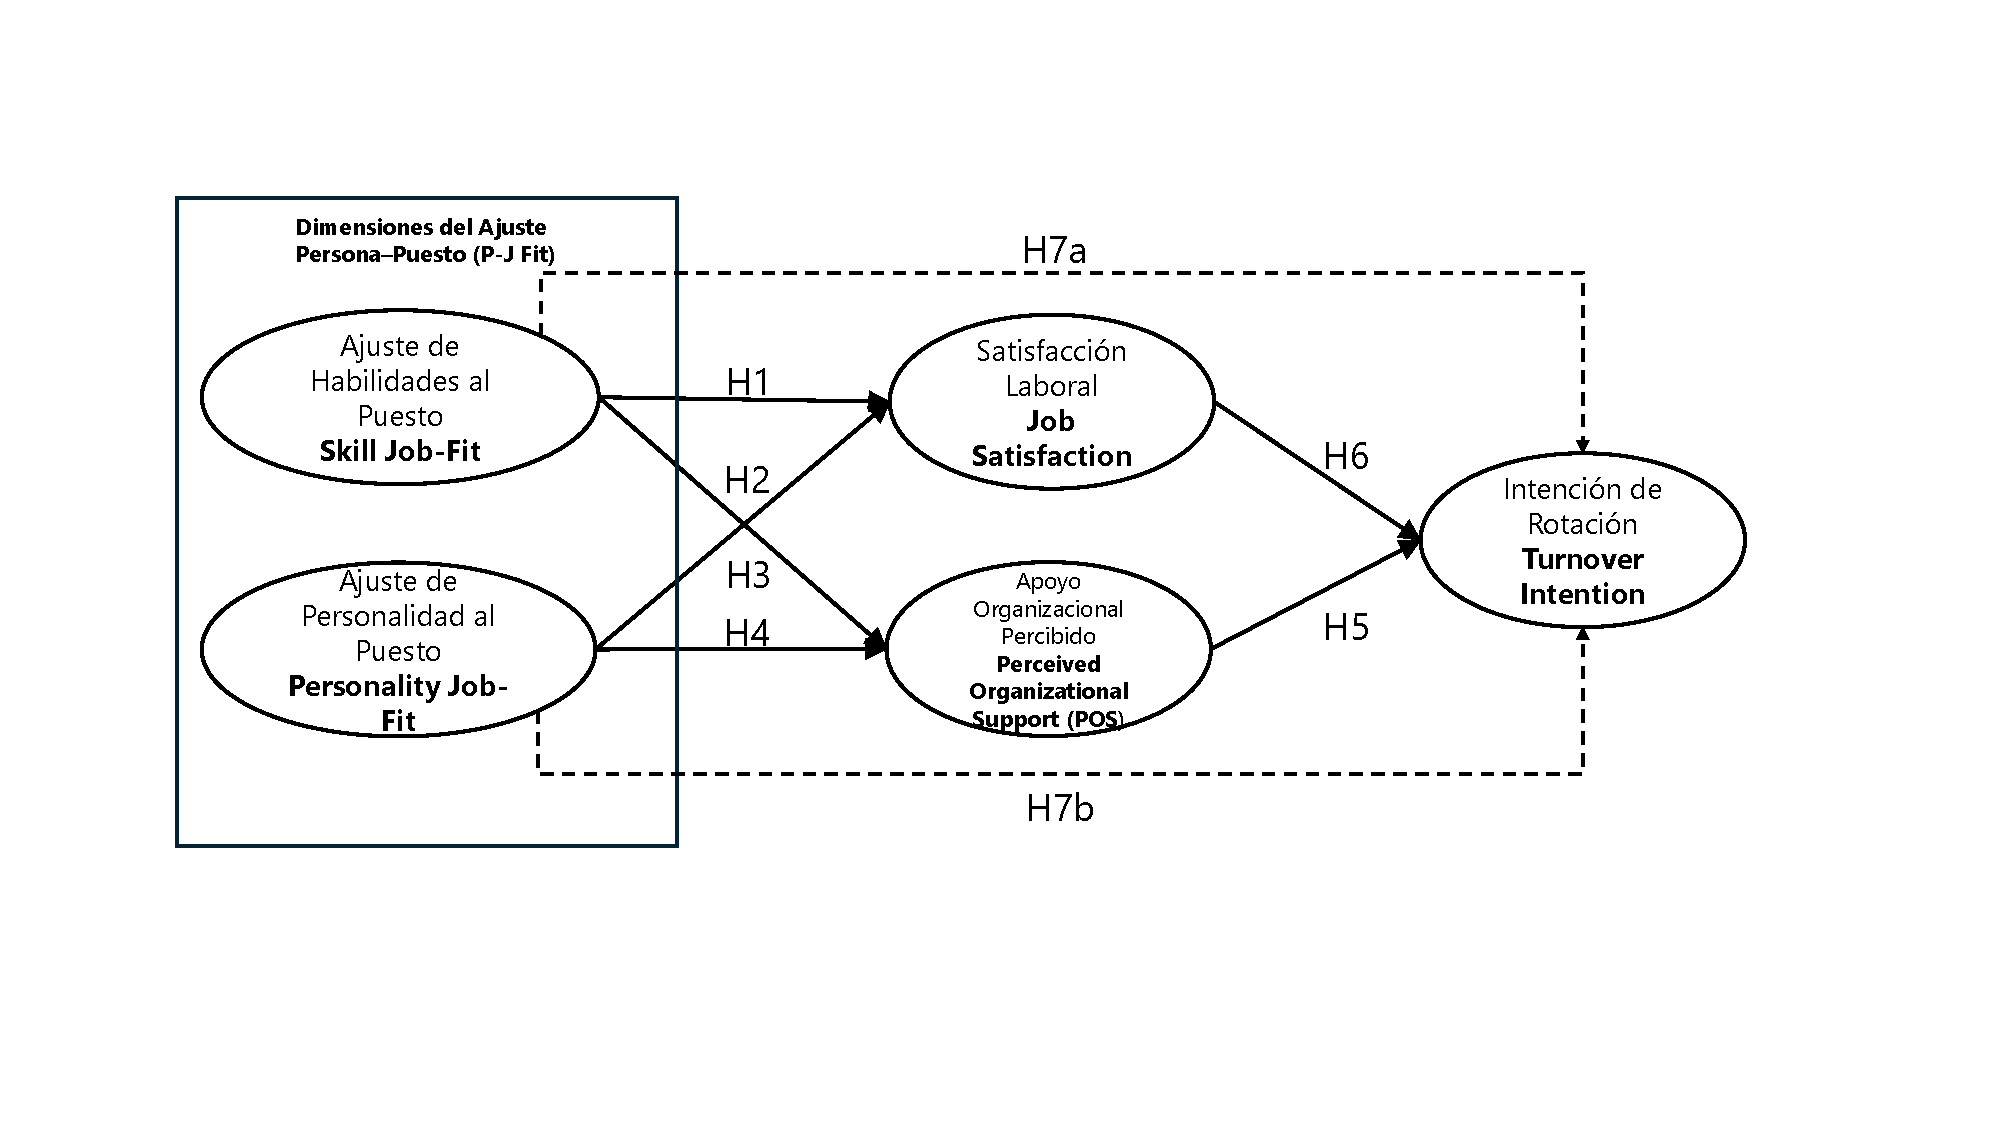
\includegraphics[width=0.9\textwidth]{figures/modelo.pdf}
  \caption{Modelo conceptual de la relación entre ajuste persona--trabajo, satisfacción laboral, apoyo organizacional percibido e intención de renuncia.}
  \label{fig:conceptual}
\end{figure}

La contrastación empírica de este modelo en una muestra de tecnólogos colombianos contribuirá a: (a) avanzar en la comprensión teórica de los mecanismos diferenciales por los cuales el ajuste técnico y sociocultural influyen sobre la intención de renuncia; (b) proporcionar evidencia empírica contextualizada que informe el diseño de estrategias de gestión del talento técnico en sectores productivos críticos para el desarrollo económico colombiano; y (c) validar instrumentos psicométricos robustos para la evaluación del ajuste persona--trabajo en poblaciones técnicas hispanohablantes, contribuyendo a cerrar la brecha de investigación organizacional en contextos latinoamericanos.